\documentclass{article}

% if you need to pass options to natbib, use, e.g.:
%     \PassOptionsToPackage{numbers, compress}{natbib}
% before loading neurips_2018

% ready for submission
% \usepackage{neurips_2018}

% to compile a preprint version, e.g., for submission to arXiv, add add the
% [preprint] option:
%     \usepackage[preprint]{neurips_2018}

% to compile a camera-ready version, add the [final] option, e.g.:
     \usepackage[final]{neurips_2018}

% to avoid loading the natbib package, add option nonatbib:
%     \usepackage[nonatbib]{neurips_2018}

\usepackage[utf8]{inputenc} % allow utf-8 input
\usepackage[T1]{fontenc}    % use 8-bit T1 fonts
\usepackage{hyperref}       % hyperlinks
\usepackage{url}            % simple URL typesetting
\usepackage{booktabs}       % professional-quality tables
\usepackage{amsfonts}       % blackboard math symbols
\usepackage{nicefrac}       % compact symbols for 1/2, etc.
\usepackage{microtype}      % microtypography
\usepackage{amsmath}
\usepackage{graphicx}
\usepackage{float}
\title{Deep Learning Homework assignment}

% The \author macro works with any number of authors. There are two commands
% used to separate the names and addresses of multiple authors: \And and \AND.
%
% Using \And between authors leaves it to LaTeX to determine where to break the
% lines. Using \AND forces a line break at that point. So, if LaTeX puts 3 of 4
% authors names on the first line, and the last on the second line, try using
% \AND instead of \And before the third author name.

\author{%
  Nzuanzu Jier \\
  10223258 \\
  \texttt{jier.nzuanzu@student.uva.nl} \\
  % examples of more authors
  % \And
  % Coauthor \\
  % Affiliation \\
  % Address \\
  % \texttt{email} \\
  % \AND
  % Coauthor \\
  % Affiliation \\
  % Address \\
  % \texttt{email} \\
  % \And
  % Coauthor \\
  % Affiliation \\
  % Address \\
  % \texttt{email} \\
  % \And
  % Coauthor \\
  % Affiliation \\
  % Address \\
  % \texttt{email} \\
}

\begin{document}
% \nipsfinalcopy is no longer used

\maketitle


\section{Vanilla RNN vs LSTM }

\subsection{Vanilla RNN in pyTorch}
\begin{itemize}
    \item Question 1 \\
    With the following basic equations we will derive the partial equations w.r.t $W_{ph}, W_{hh}, W_{hx}$.
    \begin{align*}
      h^{t} &= \tanh{\left(W_{hx}\cdot x^{t} + W_{hh}\cdot h^{(t - 1)} + b_h\right)} \\
      p^{t} &= W_{ph}\cdot h^{t} + b_{p} \\
      \mathcal{L} &= - \sum_{k = 1}^{K}  y_k \log{\hat{y_k}}
    \end{align*}
    \begin{align*}
      \frac{\partial \mathcal{L}^T}{\partial W_{ph}} &= \frac{\partial\mathcal{L}^T}{\partial \hat{y}^t} \frac{\partial \hat{y}^t}{\partial p^t} \frac{\partial p^t}{\partial W_{ph}} \\
      \frac{\partial \mathcal{L}^T}{\partial \hat{y}^t} &=  \frac{\partial}{\partial \hat{y}} -y \log{\hat{y}} + -y \frac{\partial}{\partial \hat{y}} \log{\hat{y}} \\
      &= 0 -\frac{y}{\hat{y}} \\
      &= -\frac{y^T}{\hat{y}^T} \\
      \frac{\partial \hat{y}^T}{\partial p^T} &= softmax(p^T) \frac{\partial}{\partial p^T} \\
      &= softmax(p_{i}^{T})\left(\delta_{ij} - softmax(p_{j}^{T})\right)  \\
      \frac{\partial p^T}{\partial W_{ph}} &= \frac{\partial }{\partial W_{ph}} W_{ph} \cdot h^t + \frac{\partial }{\partial W_{ph}} b_p \\
      &= -\frac{y^T}{\hat{y}^T}\cdot softmax(p_{i}^{T})\left(\delta_{ij} - softmax(p_{j}^{T})\right) \cdot h^t \\
      &= -\frac{y^T}{\hat{y}^T} \hat{y}^T \left(\delta_{ij} - \hat{y}^T \right) \cdot h^T \\
      &= - y^T \cdot \left(\delta_{ij} - \hat{y}^T \right) \cdot h^T \\
      \frac{\partial \mathcal{L}^T}{\partial W_{hh}} &= \frac{\partial\mathcal{L}^T}{\partial \hat{y}^T} \frac{\partial \hat{y}^T}{\partial p^T}  \frac{\partial p^T}{\partial h^T} \frac{\partial h^T}{\partial W_{hh}} \\
      &= \sum_{i = 0}^{T}\frac{\partial\mathcal{L}^T}{\partial \hat{y}^T} \frac{\partial \hat{y}^T}{\partial p^T}  \frac{\partial p^T}{\partial h^T} \frac{\partial h^T}{\partial h^i} \frac{\partial h^i}{\partial W_{hh}} \\
    \end{align*}
    The gradient w.r.t to the hidden state needs to be calculated up till the initial hidden unit while that of the output layer does not. With this in mind, managing memory and gradients value can be an issue in the hidden state. There is two case for this issue, either the gradient vanishes back through the initial layer or it explodes when going through time. 
    \item Question 2 See code implementation. 
    \item Question 3
    \begin{figure}[H]
      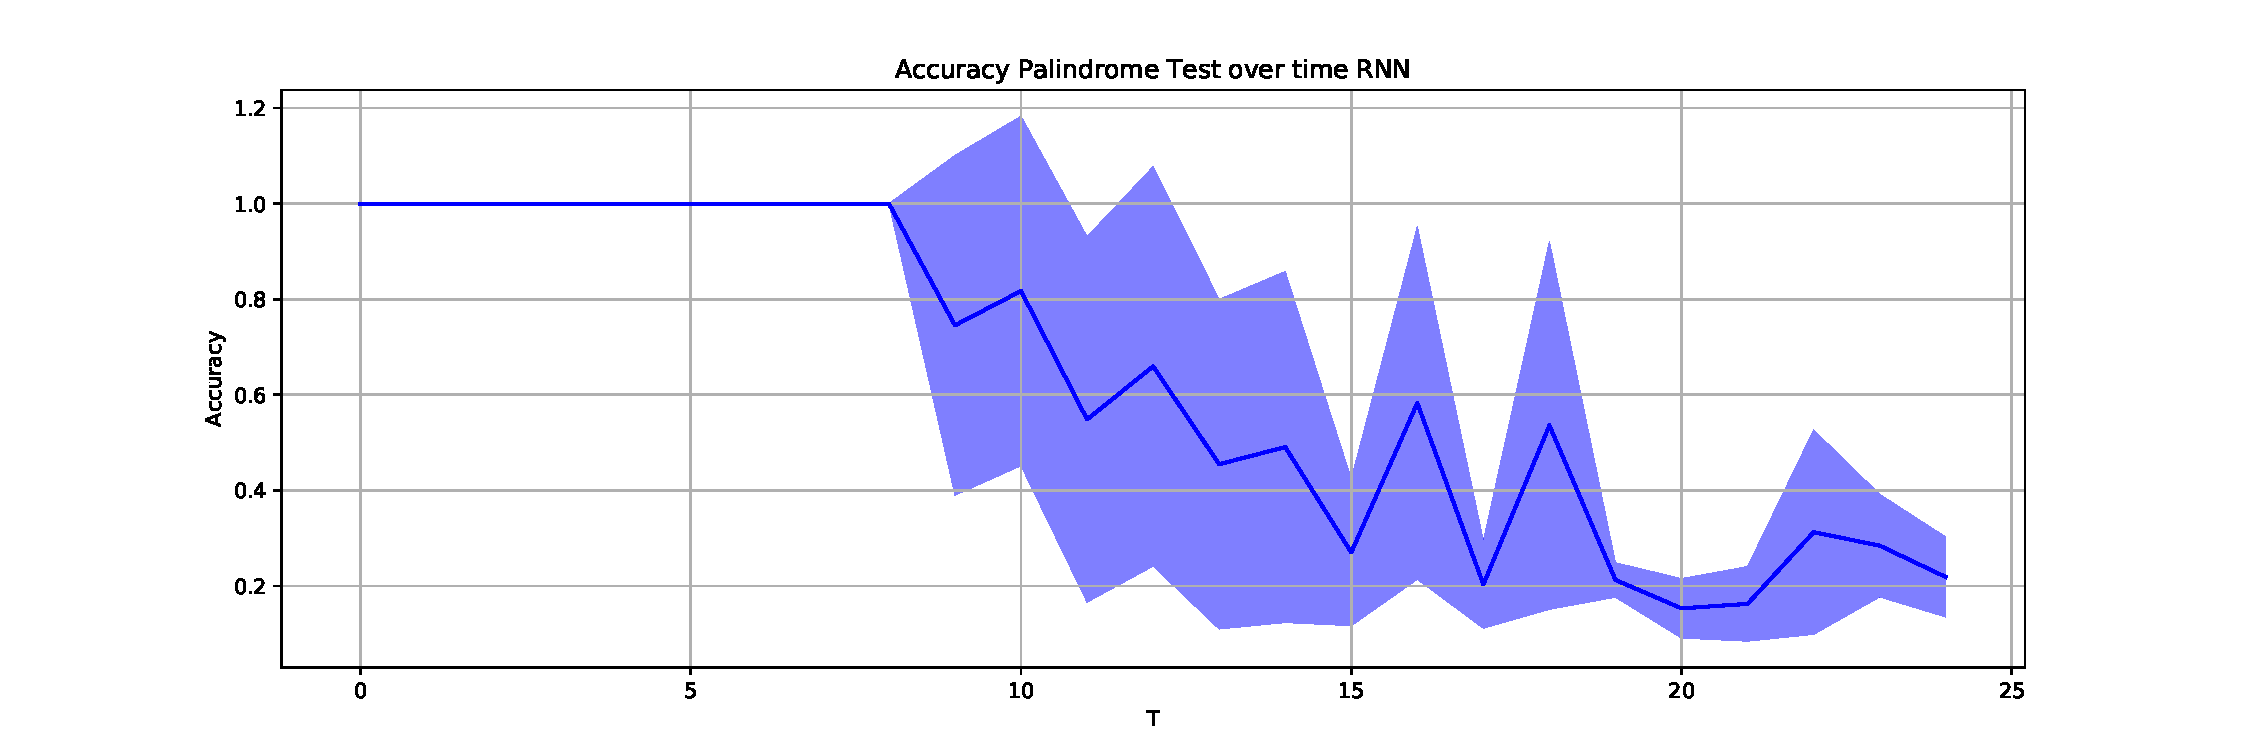
\includegraphics[width=\linewidth]{RNN_acc_.pdf}
      \caption{RNN accuracy with different seeds where we see that the accuracy deteriorate before the length 10 of a palindrome}
      \label{fig:rnn_acc}
    \end{figure}
  As we expect from Figure \ref{fig:rnn_acc}, the network is able to predict every last palindrome but it arrives at a limit where its performance deteriotate with a wide standard deviation. Eventually it arrives at a oscillating point where the memory cannot recall the complete histroy of the palindrome. Although gradient clipping has been performed, we might see the case that the gradients still vanishes and thus does not influence every next cell state to remember. 
    \item Question 4 \\
    The benefit of using RMSprop or Adam rather than SGD is that the previous optimizer take the momentum into account during training, while SGD not well tuned might oscillate to find the optimal solution. Moreover SGD updates its step according through the loss value  back-propagated, while the aforementioned optimizer utilize adaptive learning rates where there is a global learning rate and a targeted learning rate for each weight that changes during training depending on the sign between current gradient and velocity of that weight. Differently put, adaptive learning rate ensure that the change in signs of the weights during training will influence if the training is approaching a (global) minimum.  
\end{itemize}
\subsection{Long Short Term Memory (LSTM) in pyTorch}
\begin{itemize}
  \item Question 5 \\
  The forget-gate is responsible to ensure and inspect the usefulness of the information entering the cell over time, so it scales numerically the usefulness between $0$ and $1$ and thus behaving as switch. 
  The input-gate also needs to evaluate the usefulness of the current input and registering it to the cell state. This gate also behaves as a switch due to the sigmoid function output. The output-gate,finally needs to evaluate the information usefulness of the system to pass to the next cell state.  The output gate generates candidate with $\tanh$ activation function according to the forget and input gate, the effect of a different activation between $-1, 1$ is either to excite or dampen the activation for the next cell state with information. 

  We know from the definition that there are four different weight matrices depending on the input, hidden units and biases. Thus we will require the sum of the following; for an input matrix with dimension $d x n$, weights of hidden units $ n x n$ and biases vectors $n$. This is $4 *(d x n) + 4*( n x n) + 4 * n$  trainable parameters that are needed for training. 
  \item Question 6
  \begin{figure}[H]
      \centering
      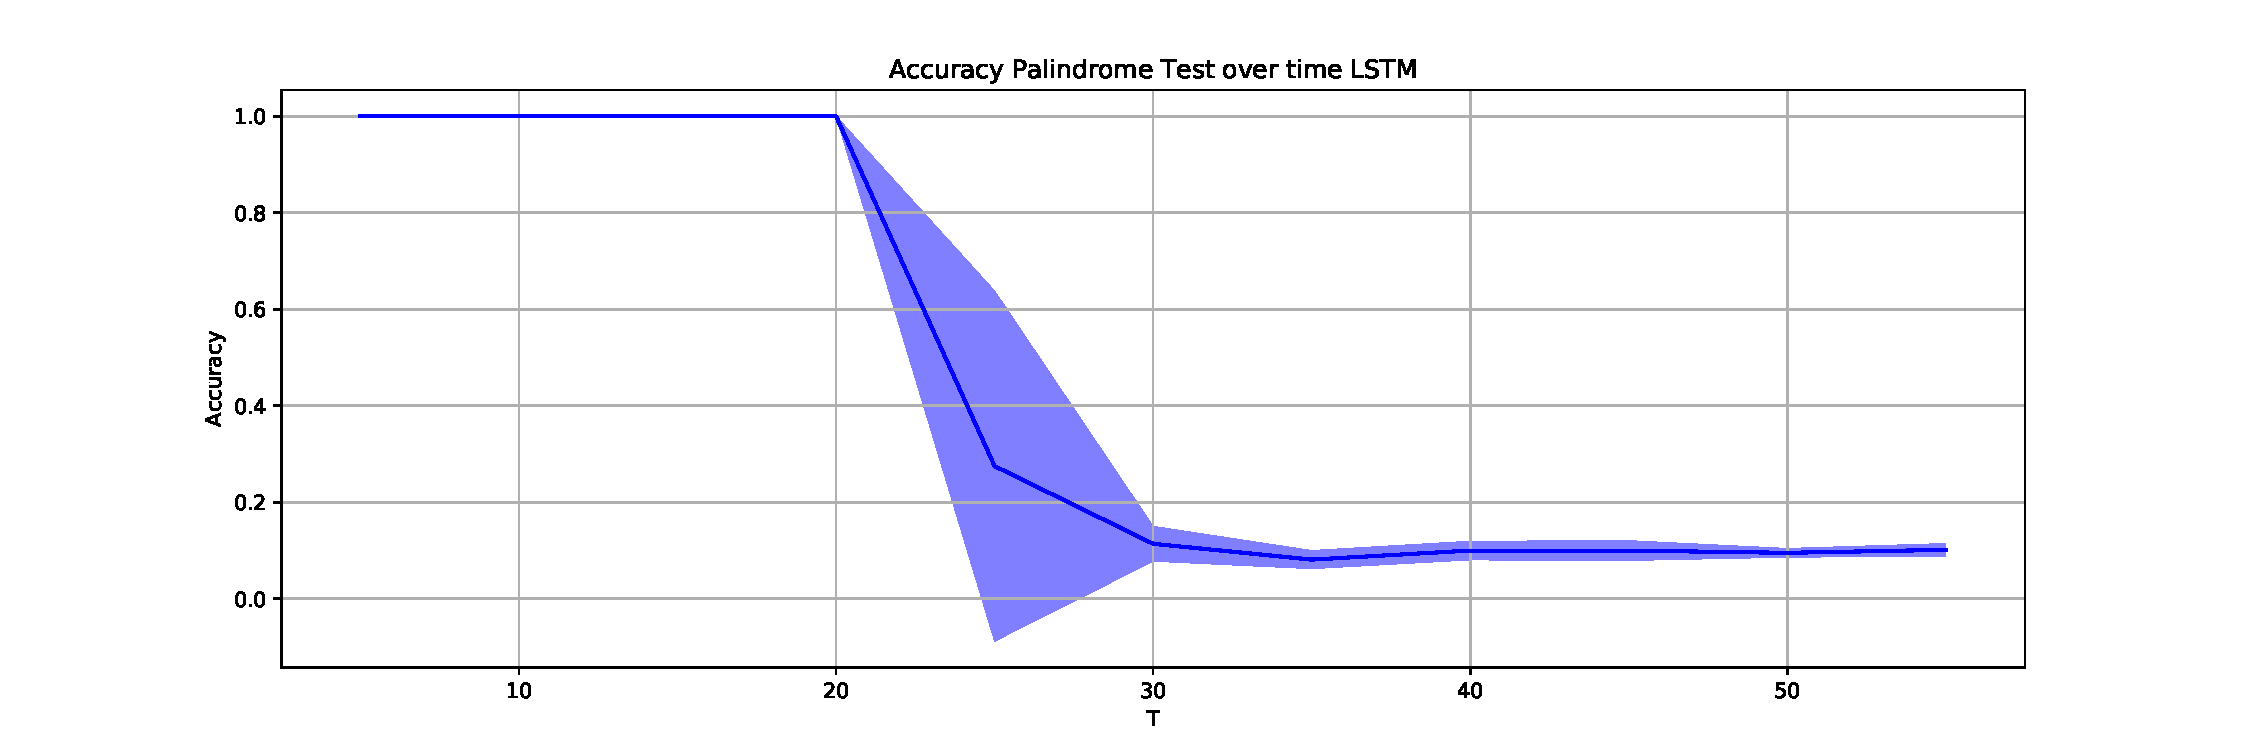
\includegraphics[width=\linewidth]{LSTM_acc_.pdf}
      \caption{The accuracy of LSTM where we observe a decrease of accuracy later than a regular RNN}
      \label{fig:lstm_acc}
  \end{figure}
  It is from Figure \ref{fig:lstm_acc} quite the opposite compared to Figure \ref{fig:rnn_acc} where we see now a delay in deterioration after a certain length of data input. This figure has been run with the default values as the previous figure. The same behaviour as the RNN counterparts occur, but quite faster between length $20 - 50$. 
  \item Question 7
  \begin{figure}[H]
      \centering
      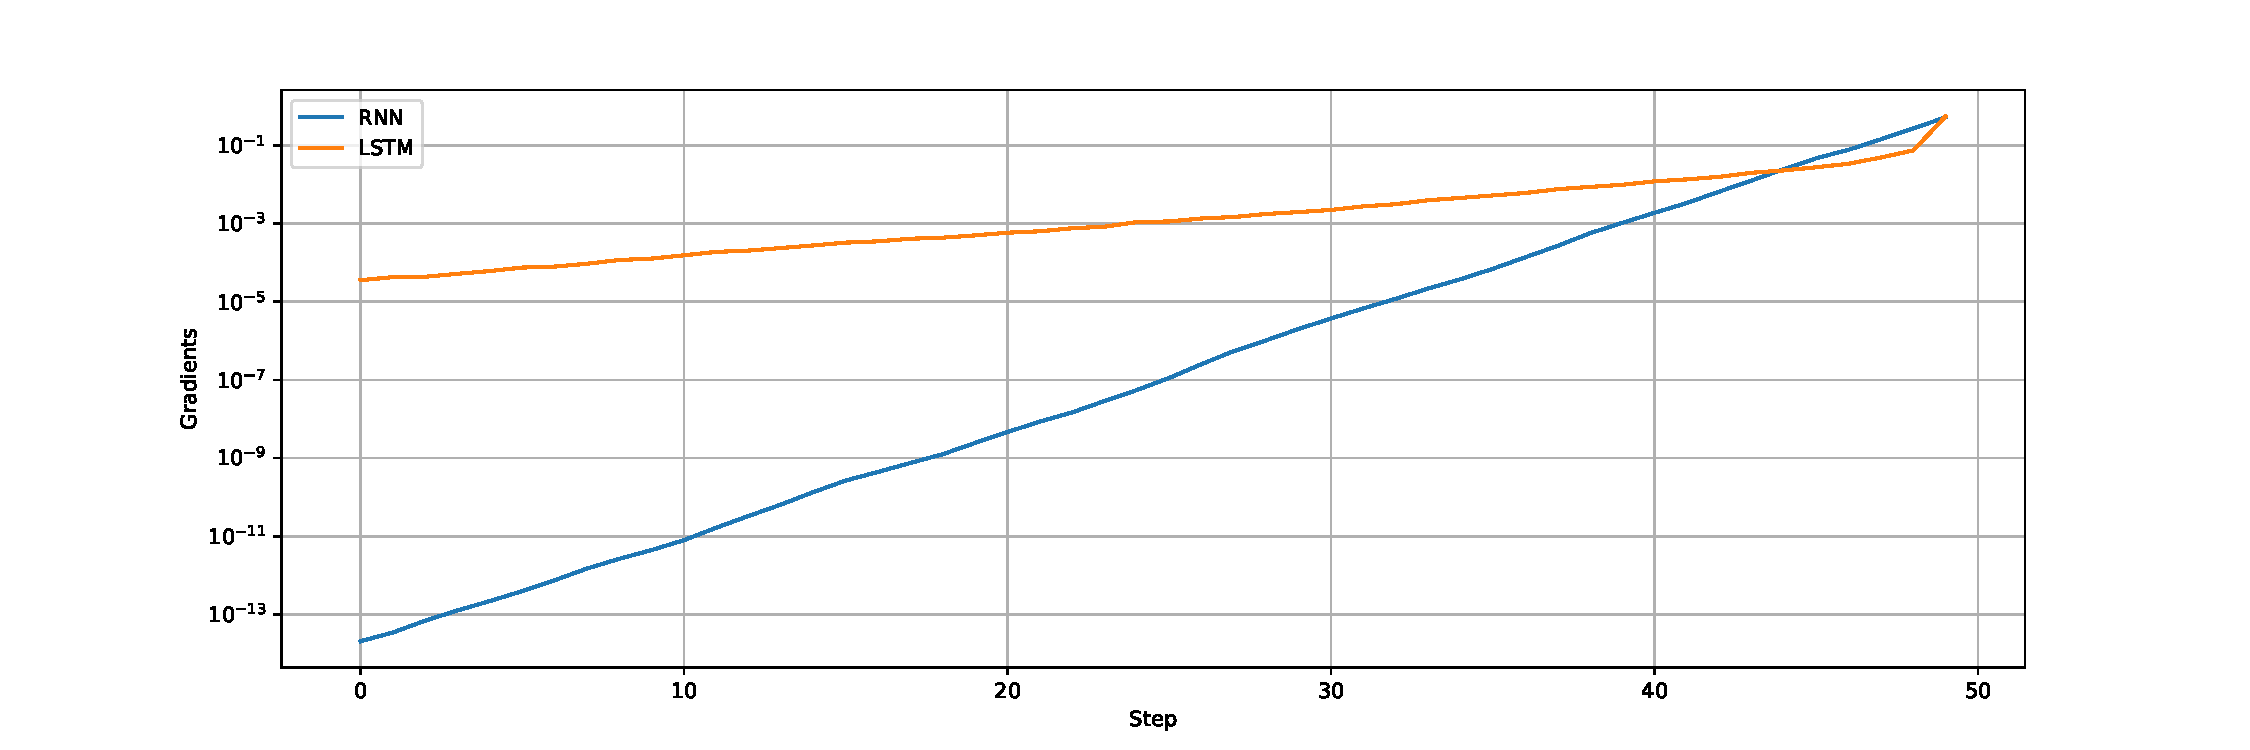
\includegraphics[width=\linewidth]{hidden_gradients.pdf}
      \caption{We see when we observe the hidden layers that the LSTM grows exponentially slower than the regular RNN }
      \label{fig:hidden_lstm_rnn}
  \end{figure}
\end{itemize}
When we inspect the hidden state of both networks we exactly encounter the same delay behaviour in decay, where the LSTM decays slower than the RNN.  
\section{Recurrent nets as Generative Model}

\begin{itemize}
  \item Question 1 \\
  For this assignment we chose to keep the default value and only use the RMSprop optimizer with twenty epochs as the choice of the optimizer seems working well for the model as its well suited as it has an adaptive learning and uses momentum to update the gradients between layers. This is quite important for a network where there are more gradient update within the cells as between the cells.  
  \item Question 2 See data outputs and code
  \item Question 3 see above
  \item Question 4 see above
\end{itemize}

\section{Graph Neural network}

\subsection{GCN Forward Layer}
\begin{itemize}
  \item Question 1 \\
  With every node present, the layer contains informations of the nodes and their neighbours that is encoded in the adjencecy matrix. As passing from one layer to another the information of the neighbours is used to traverse the graph. 
  \item Question 2 \\
  In a graph where there is no edge between the nodes for example see Figure 2 in the assignment, with one layer it will not make it possible to pass the information from example node $b$ to $e$. To resolve this issue, we should create a network with as many layer as the diameter of the graph. 
  \item Question 3
  \begin{align*}
  \tilde{A}= \left(\begin{matrix}1&1&0&0&1&1\\1&1&1&1&0&0\\0&1&1&1&0&0\\0&1&1&1&0&1\\1&0&0&0&1&1\\1&0&0&1&1&1\end{matrix}\right)
  \end{align*}
  \item Question 4 \\
  So, we require three updates, because there are two edges between these nodes to be traversed. 
\end{itemize}

\subsection{Applications of GNN}
\begin{itemize}
  \item From \cite{shen2018person} we see that the re-indentification problem in the computer vision domain an attempt to resolve it with the aid of Graph Neural Network.
  \item Furthermore, we see that \cite{prates2019learning} uses Graph Neural network to solve an NP-Complete problem as the travelling salesman problem. 
\end{itemize}


\subsection{Comparing GNN and RNN}
\begin{itemize}
  \item Question 1 \\
  Using text translation with RNN would be very suitable but using the text to understand context, a GNN will likely be very suitable where perhaps every sentence or paragraph could be a node and each next sentence or paragraph could be connected with an edge. This choice of representation would make it very useful to understand the overall structure, this could act as a viable memory compared to the memory issue a regular RNN network would face if the task would be context understanding. With complex data representation where connection in the building blocks are necessary, a GNN would be very suitable and flexible to understand such data. Similarly, sequences which could have some inherently pattern as music, dance, sentences a representation with an RNN network can be very suitable.
  \item Question 2 \\
  As we have already learned, images are complex data structures to process in an neural network. This recent article by \cite{liang2016semantic} combines an LSTM with a graph network representation of an image in order to understand segmentation of an image. Each pixel as node and the spatial relation between the nodes as edges, the updates are confidence driven where the emphasis is on different semantic correlations with neighbouring nodes. 
\end{itemize}
 
\bibliography{reference.bib}
\bibliographystyle{apalike}


\end{document}
